\documentclass[12pt]{article}
  \usepackage{graphicx}
  \graphicspath{{images/}}

\pagestyle{empty}
\setcounter{secnumdepth}{2}

\topmargin=0cm
\oddsidemargin=0cm
\textheight=22.0cm
\textwidth=16cm
\parindent=0cm
\parskip=0.15cm
\topskip=0truecm
\raggedbottom
\abovedisplayskip=3mm
\belowdisplayskip=3mm
\abovedisplayshortskip=0mm
\belowdisplayshortskip=2mm
\normalbaselineskip=12pt
\normalbaselines

\begin{document}

\vspace*{0.5in}
\centerline{\bf\Large Design Document}

\vspace*{0.5in}
\centerline{\bf\Large Team PB-PJ}

\vspace*{0.5in}
\centerline{\bf\Large 18 March 2018}

\vspace*{1.5in}
\begin{table}[htbp]
\caption{Team PB-PJ}
\begin{center}
\begin{tabular}{|r | c|}
\hline
Name\\
\hline\hline
Matthew Ferderber\\
Matthew Dugal\\
Mylene Haurie\\
Viktoriya Malinova\\
Eric Morgan\\
Artem Khomich\\
Kai Nicoll-Griffith\\
Maxmilien Malderle\\
\hline
\end{tabular}
\end{center}
\end{table}

\clearpage

\section{Introduction}

The design document provides a detailed view into the design of the application
and justifies the various design decisions made by the programmers. The architecture design section
provides a high-level view of the architectural choices while the detailed design section
focuses on the detailed implementation of the architecture and all aspects of the system.
The Subsystem Interface Specification describes the two major Subsystems of the
application and all of their components.

\section{Architectural Design} \label{sec:arch}

The My Money application uses the Model View Controller architecture to seperate code into
logical components (models, view, and controllers).

\subsubsection{Models}

Models are used to provide a simple interface for the data used by the application uses.
Whenever changes are made in the model (by the controller), the view is notified and updated.

\subsubsection{Views}

Views are the visual representation of the models. Any data that needs to be shown to the user is
given to the view through models and is updated when changes are made to the model.
The view can also be updated by the controller. When an action is performed by the user,
the view delivers the action to the controller which provides the logic behind the requested
action.

\subsubsection{Controllers}

Controllers provide the logic that allows for interaction between the user and the application.
When an action is performed by the user it is relayed from the view to the responsible controller.
The controller uses its internal state to decide what the outcome of the action should be.
When the outcome is decided, the controller can update which view the application displays
or the model that is bound to the current view.

\subsubsection{Benefits}

MVC provides many benefits for the application. It allows for seperation of display, logic and 
data access into components. Because components are seperated, the same portions of the project
can be worked on by multiple people in parallel. Without having to worry about the status of the whole
application, a view can be updated to display data differently, 
the model can be modified to contain more data, and the controller can
handle new actions.


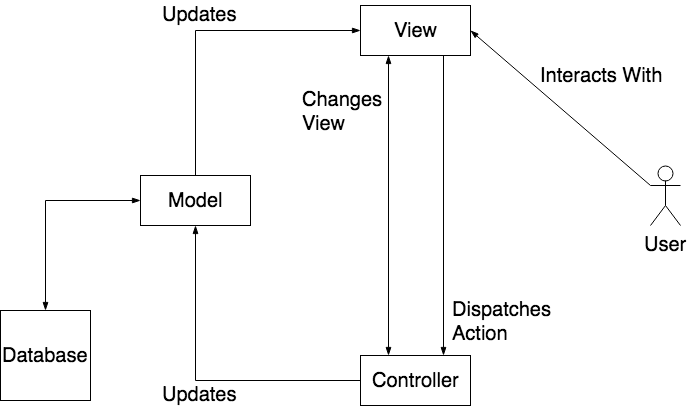
\includegraphics[scale=0.7]{archdesigndiagram}\\

This diagram shows the interaction between the models, views, and controllers.
As described above, the user interacts with the view which displays data from the model.
The view can send actions to the controller which prompts an update of the view/model.
The model (and Data Access Objects) interact with the database to update and retrieve data.

\subsection{Architectural Diagram}
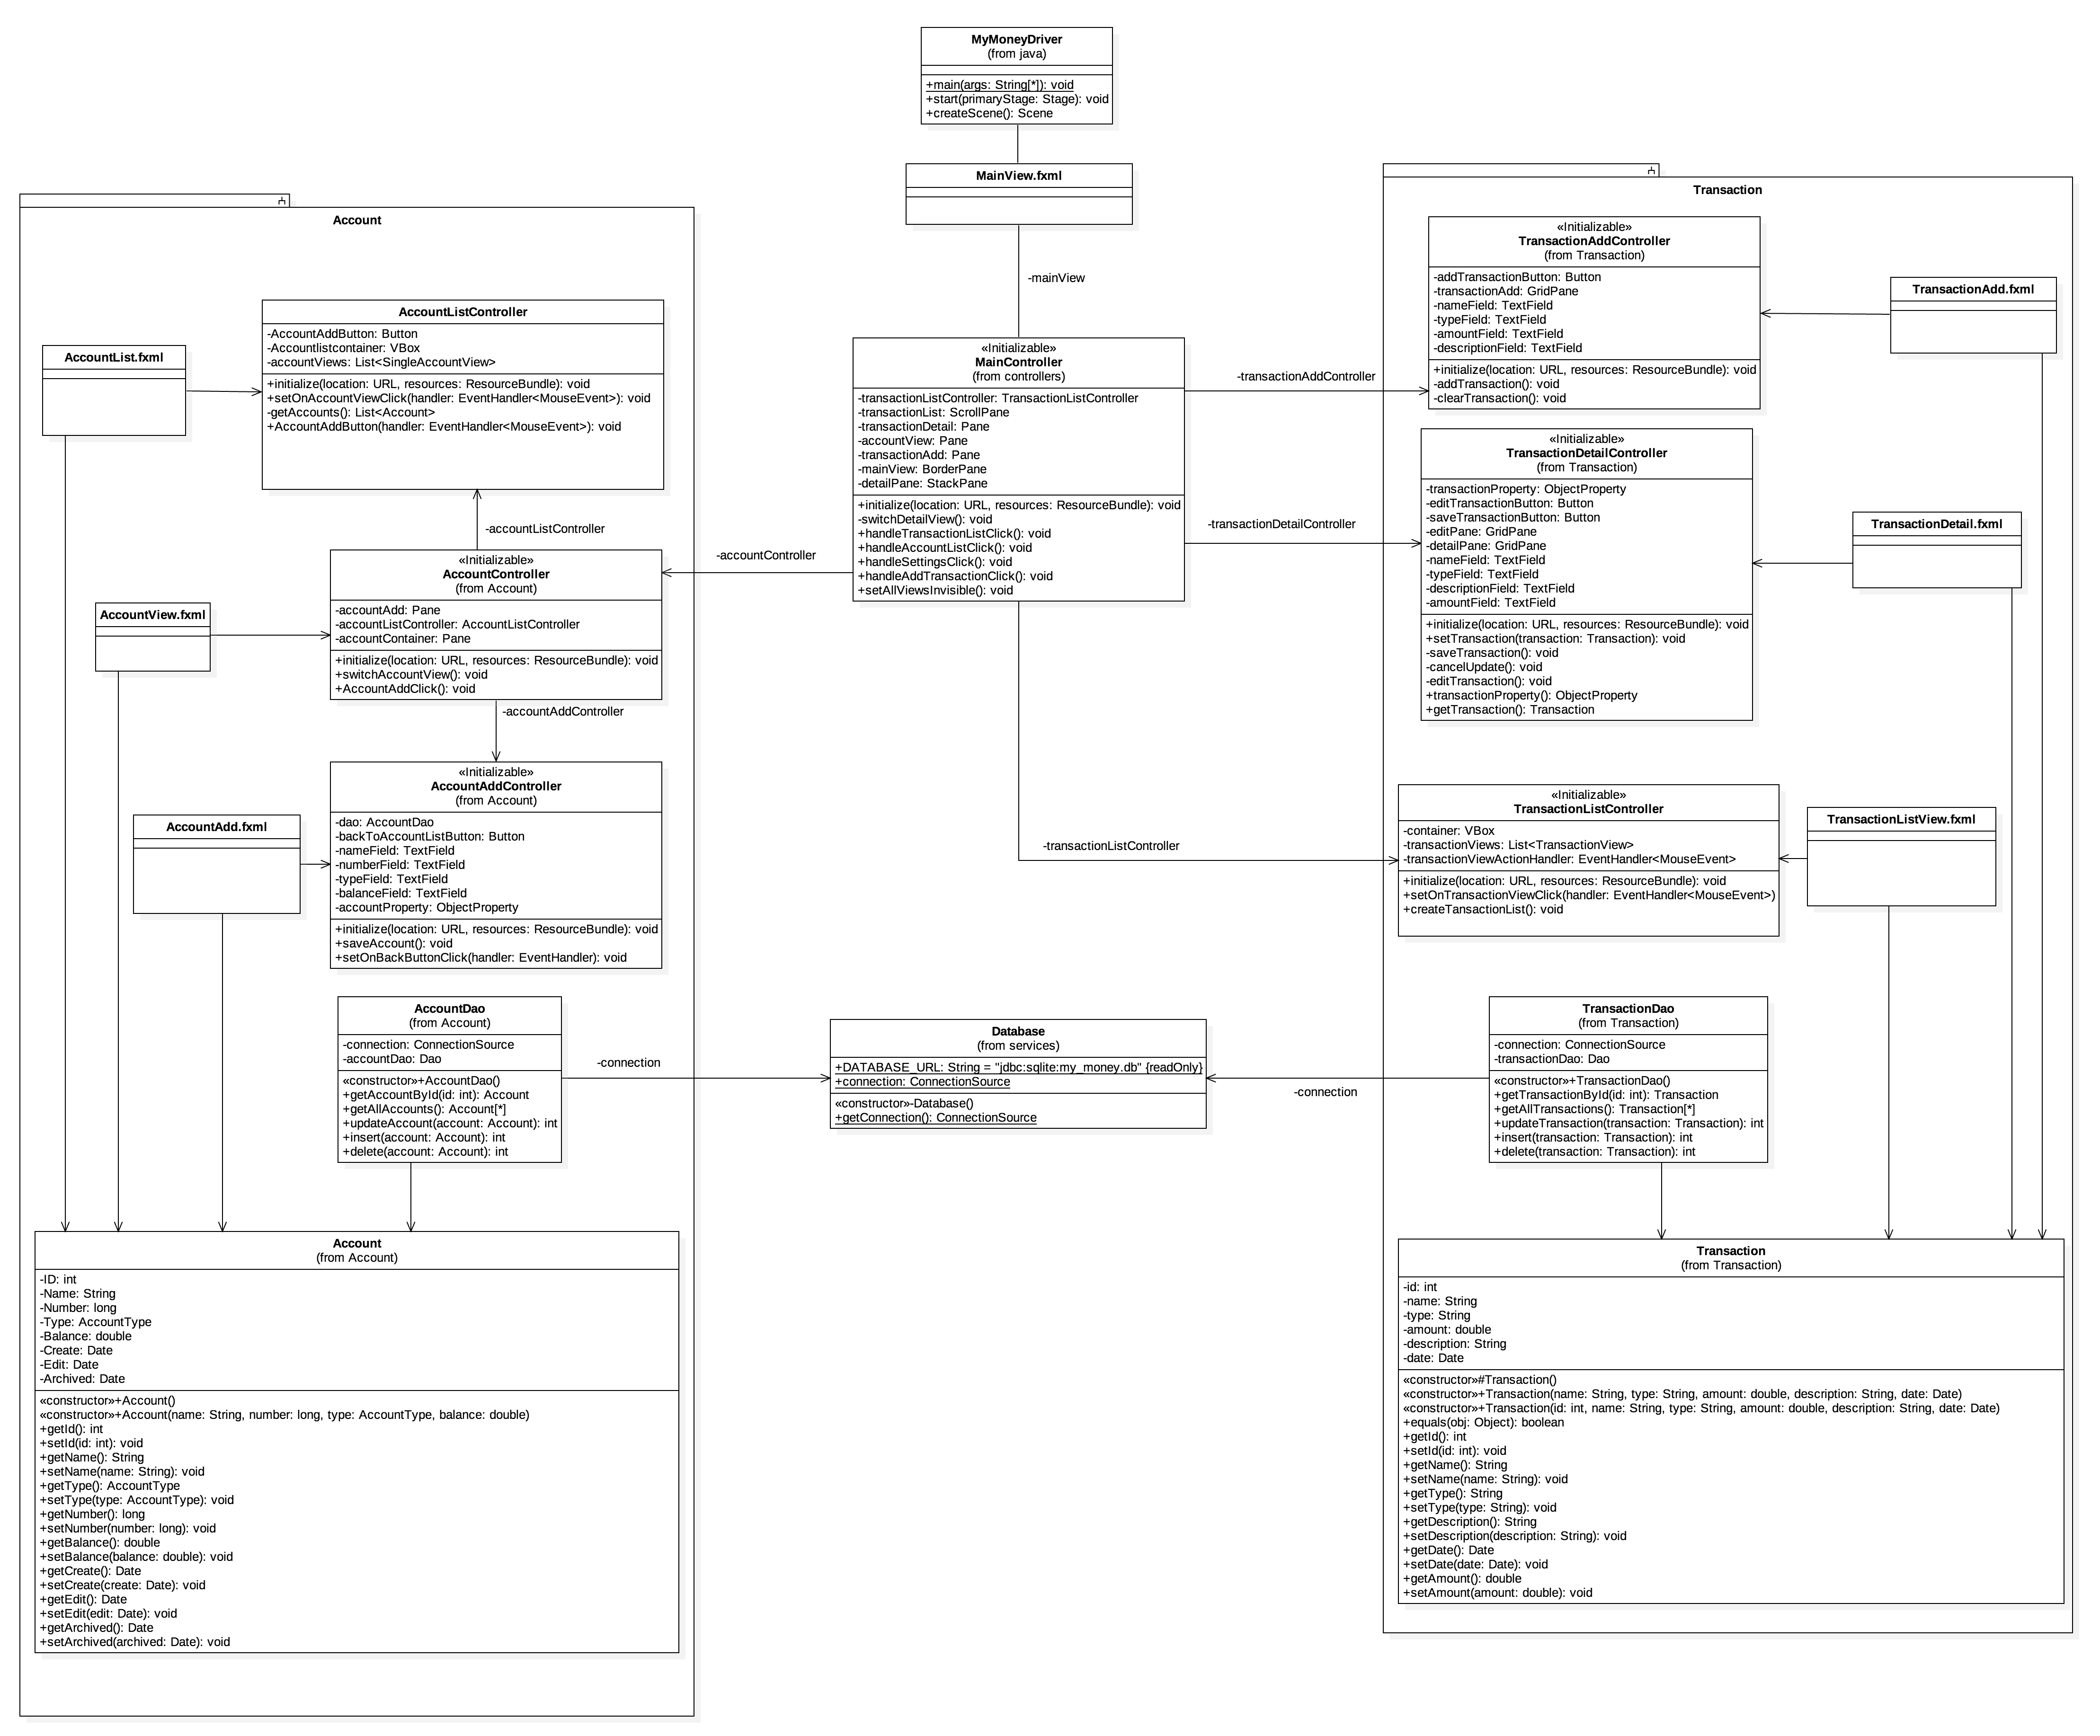
\includegraphics[scale=0.12]{classdiagram}

The MVC architecture of the system allows for the project to be modularized
into multiple submodules. This diagram shows the Account and Transaction
submodules which make up the main functionality of the system. Organizing the system
like this allows for major re-use of components such as the models (Account and Transaction)
which are used for every view in their respective module.

\subsection{Subsystem Interface Specifications}

\subsubsection{Account Subsystem Interface}

The Account Subsystem is the system that allows the user to manage
their accounts used to store transactions. Accounts are typically used
to represent real bank accounts or similar real-world accounts that transactions
can take place with. There are three main
views associated with the account system. The detailed view, list view, and add view.

\subsubsection{Account List View}

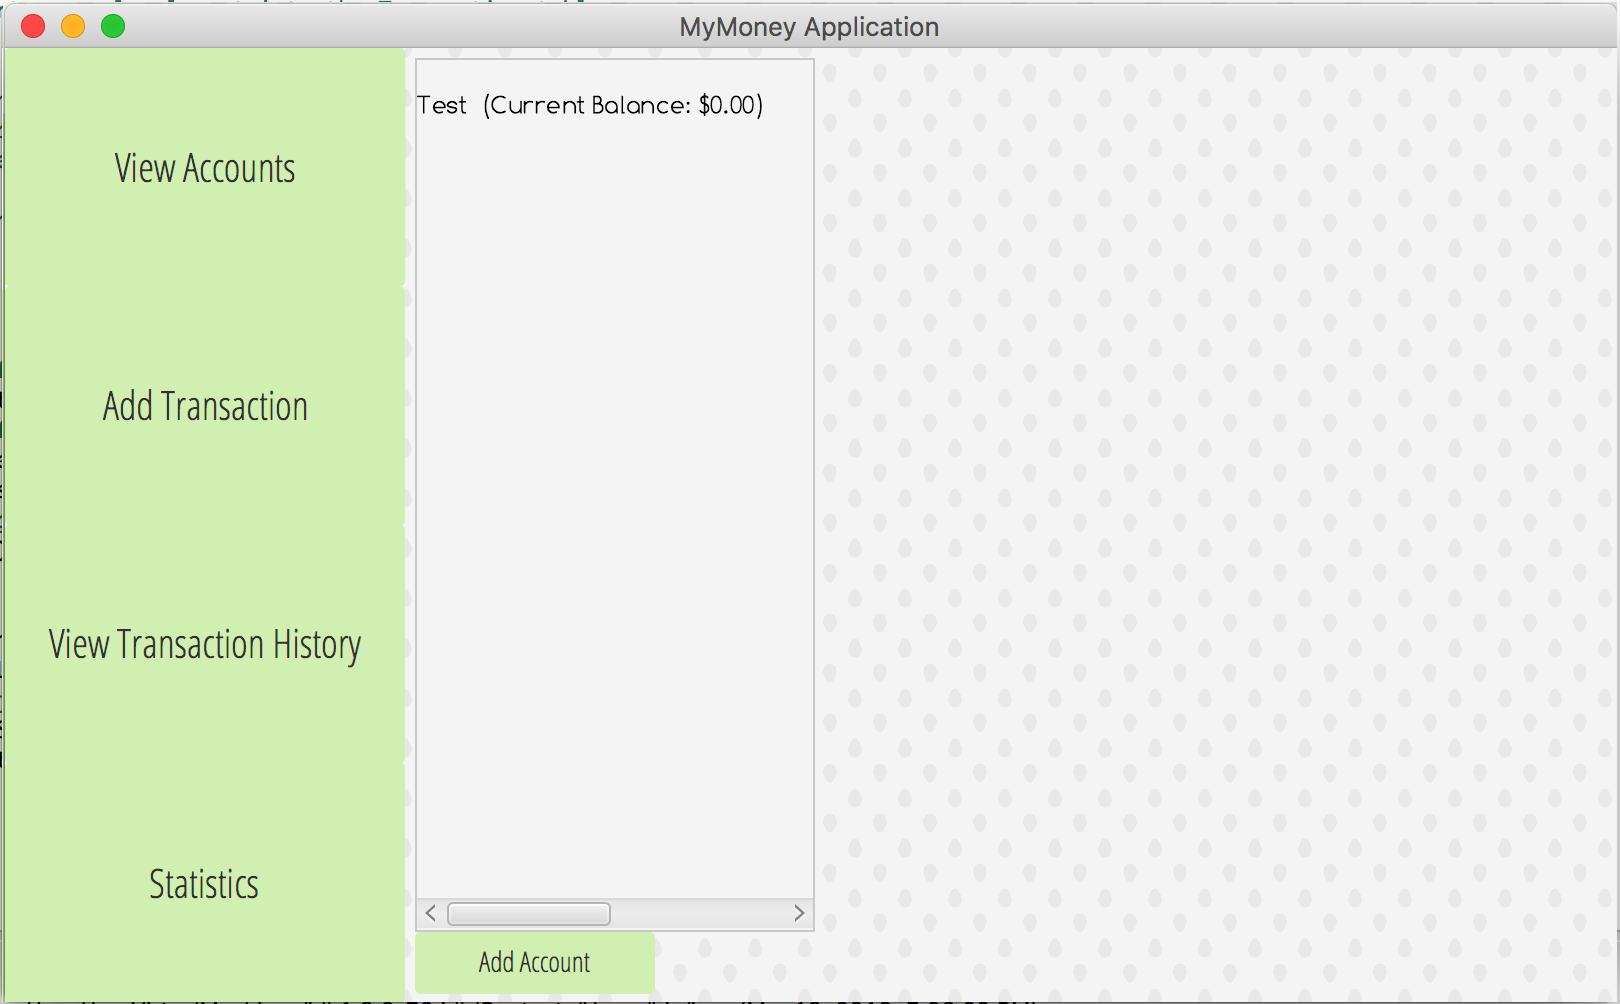
\includegraphics[scale=0.2]{accountlist}

The Account list is responsible for showing an up-to-date list of all of
the accounts in the application. From the Account List, the user can enter
into the Detailed view and the Add view by double clicking on a list item
or clicking on the add Account button respectively.\\

The AccountListController is used to manage switching between
views related to the Account List (as seen in the class diagram). 
The AccountListController will either call the 
``AccountViewActionHandler'' or the ``AccountAddClick'' event handlers
when the view is interacted with by the user.


\subsubsection{Account Detailed View}

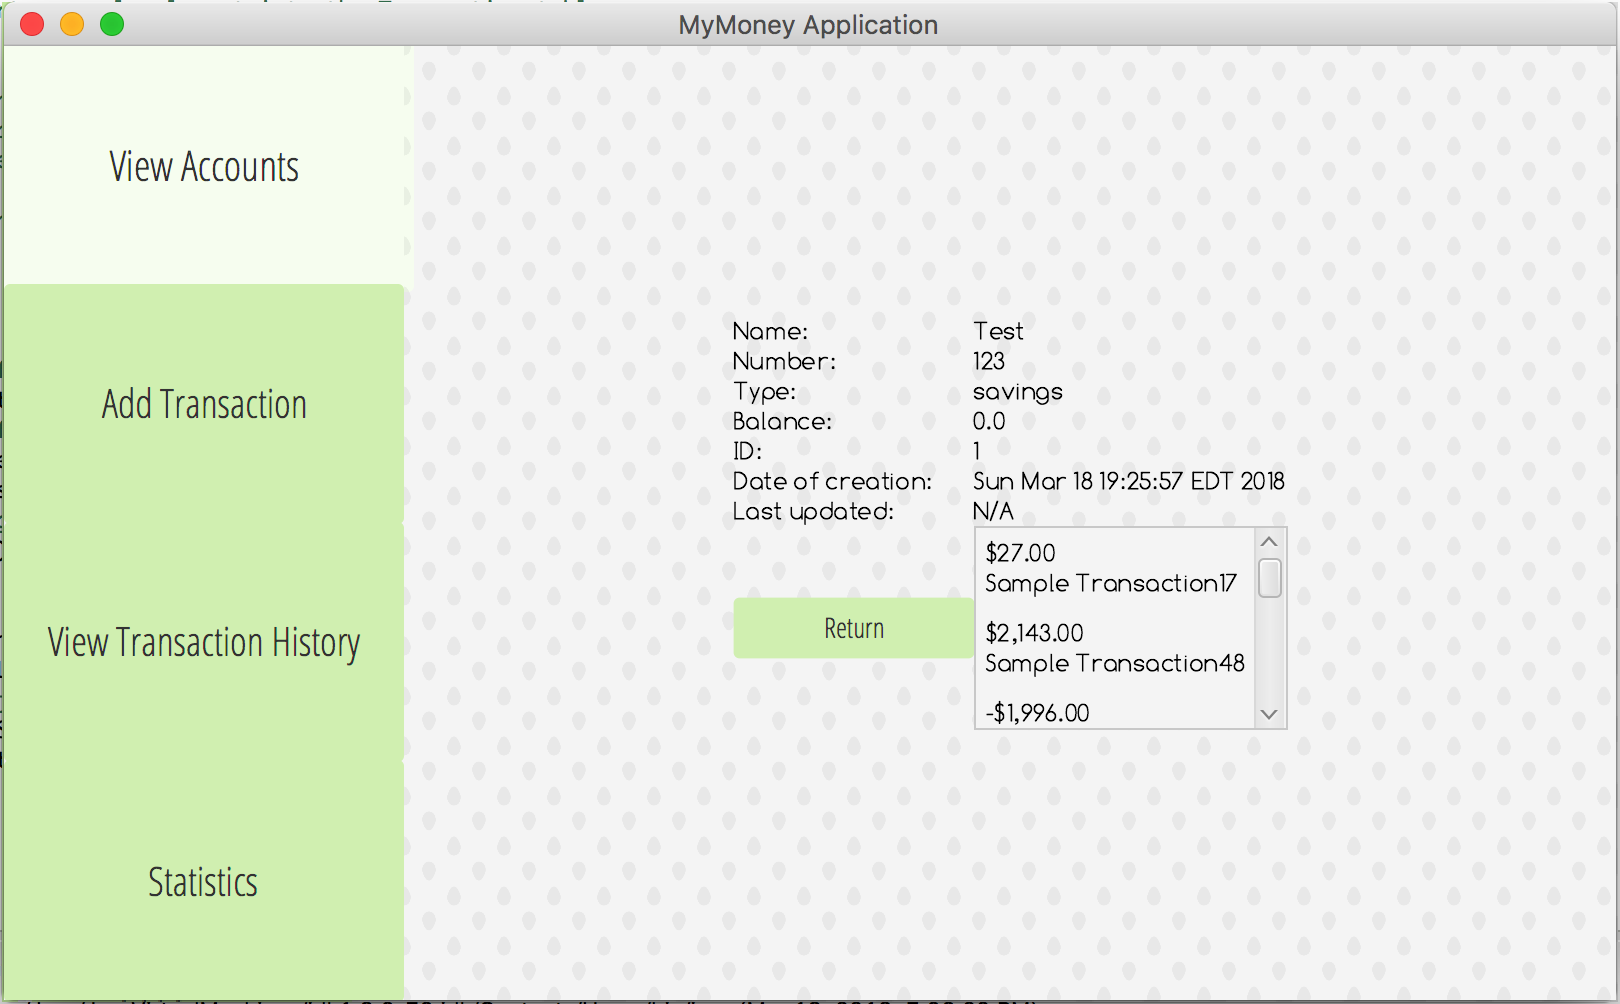
\includegraphics[scale=0.2]{accountdetail}

The Detailed view represents one Account and is responsible for
showing all of the details associated with the selected account. 
Due to the informational nature of the detail view, there are no actions
the user can perform in the view.

\subsubsection{Account Add View}

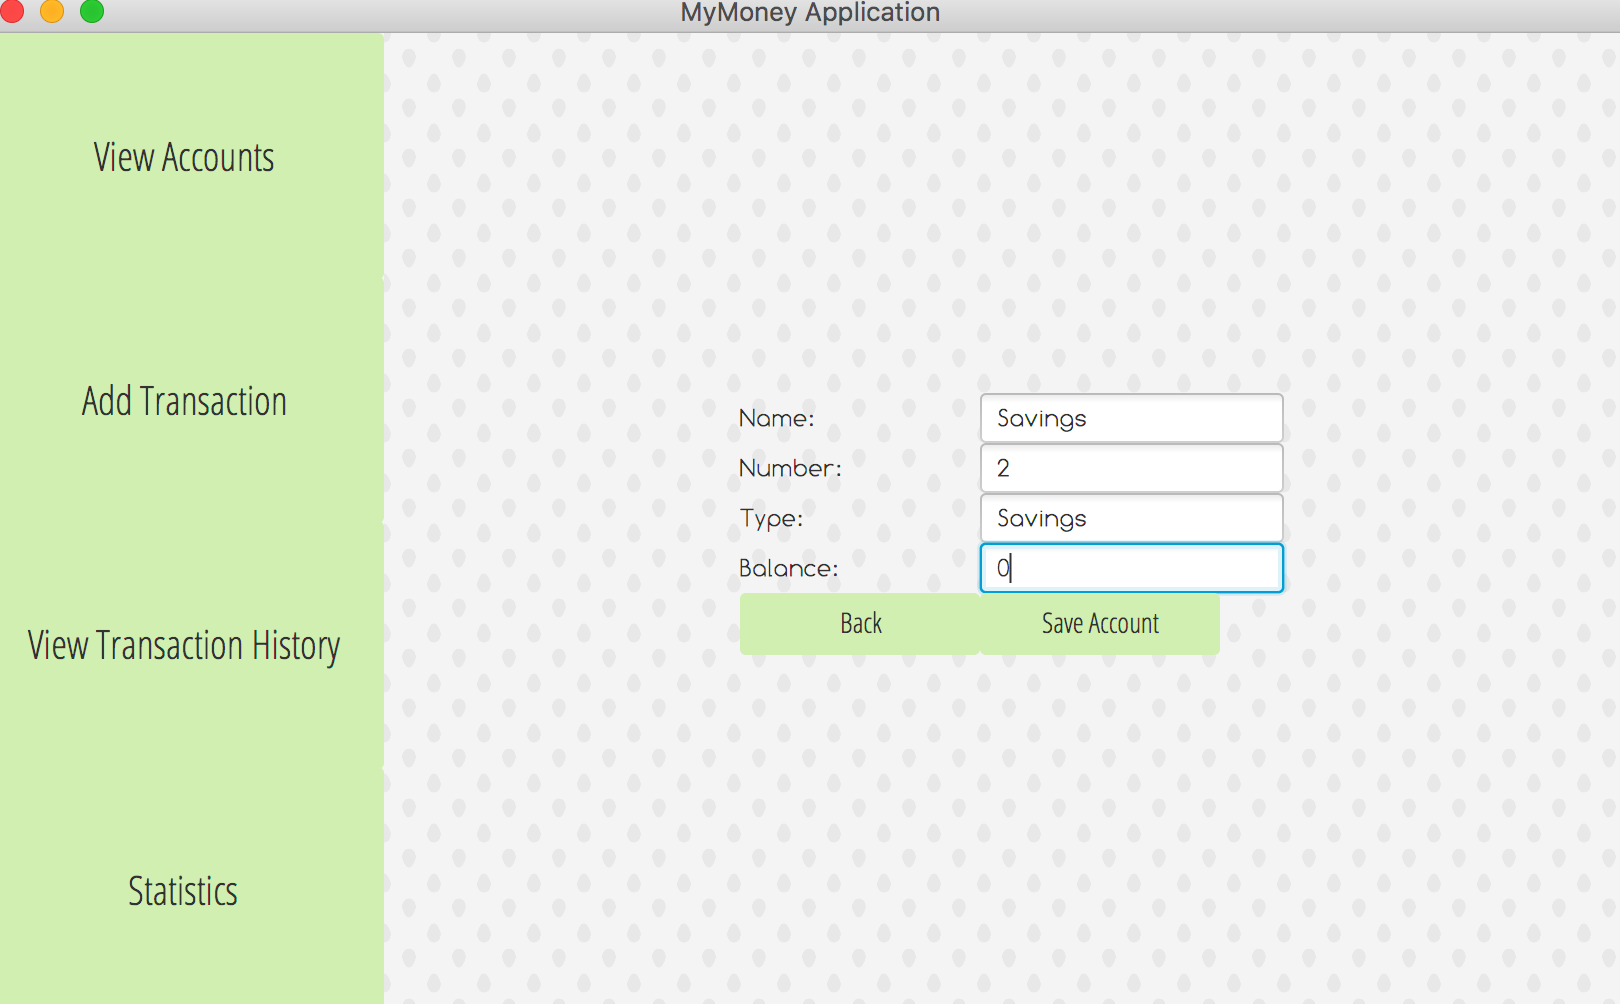
\includegraphics[scale=0.2]{accountadd}

The Account Add view is used for creating new accounts in the system.
When creating an account, the user enters the relevant account details
(Account name, number, account type, and initial balance).\\

When the user saves the account, the AccountAddController is passed the
action by the AccountAddView. The ``saveAccount'' method is called
which retrieves the new accounts details from the view and inserts it into the
database using the AccountDAO. Once inserted, the user is returned to the
Account List view where they can continue interacting with the system.

\subsubsection{Transaction Subsystem Interface}

The Transaction Subsystem allows the user to add, delete, and edit
transactions associated with an account. Transactions represent real-world
currency transactions and have a Name, type, amount, description, and 
associated account. Transactions have three main views. The Transaction list view,
detail view, and add view.

\subsubsection{Transaction List View}

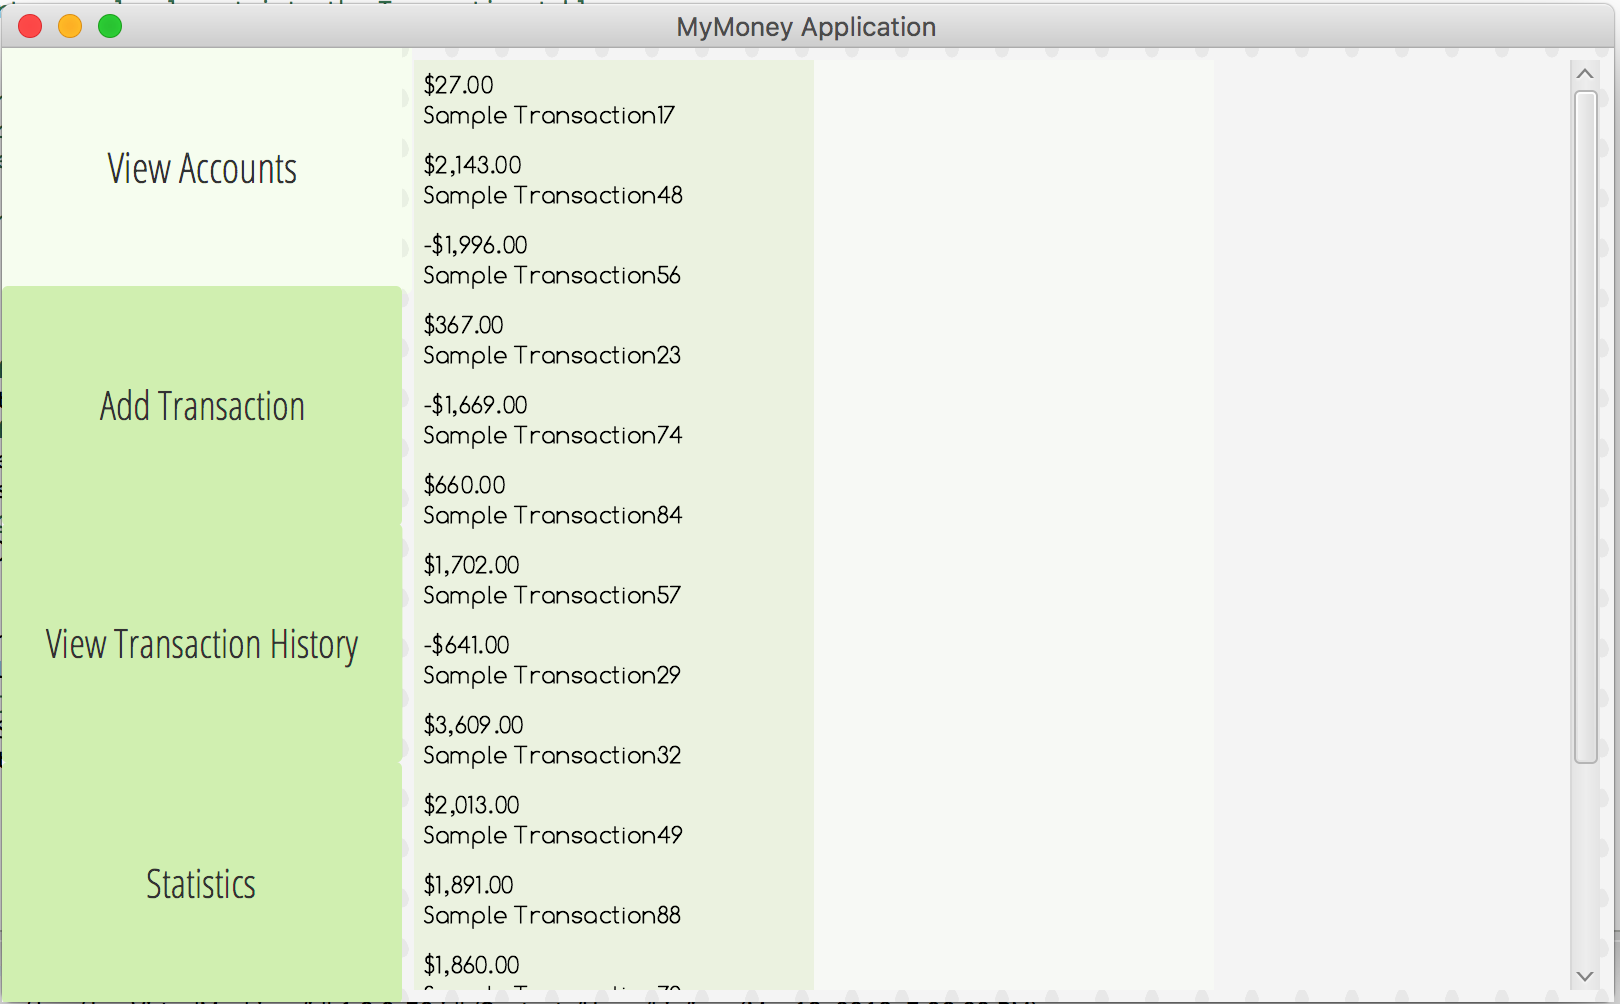
\includegraphics[scale=0.2]{transactionlist}

The Transaction List is used to show all of the transactions and a brief
description of what they represent (amount and name). The list is
expandable using the scroll wheel which allows the user to view all of
their transactions sorted by date in descending order.\\

From the Transaction List, the user can click on any transaction to be
brought to the Detailed Transaction View. When a transaction is clicked,
the event handler passed to the TransactionListController by the MainController
is executed which the main view uses to decide which transaction to create in the
TransactionDetail. In this way, the MainController acts as a dispatcher which takes
events and handles the high-level event of displaying different views.

\subsubsection{Transaction Detail View}
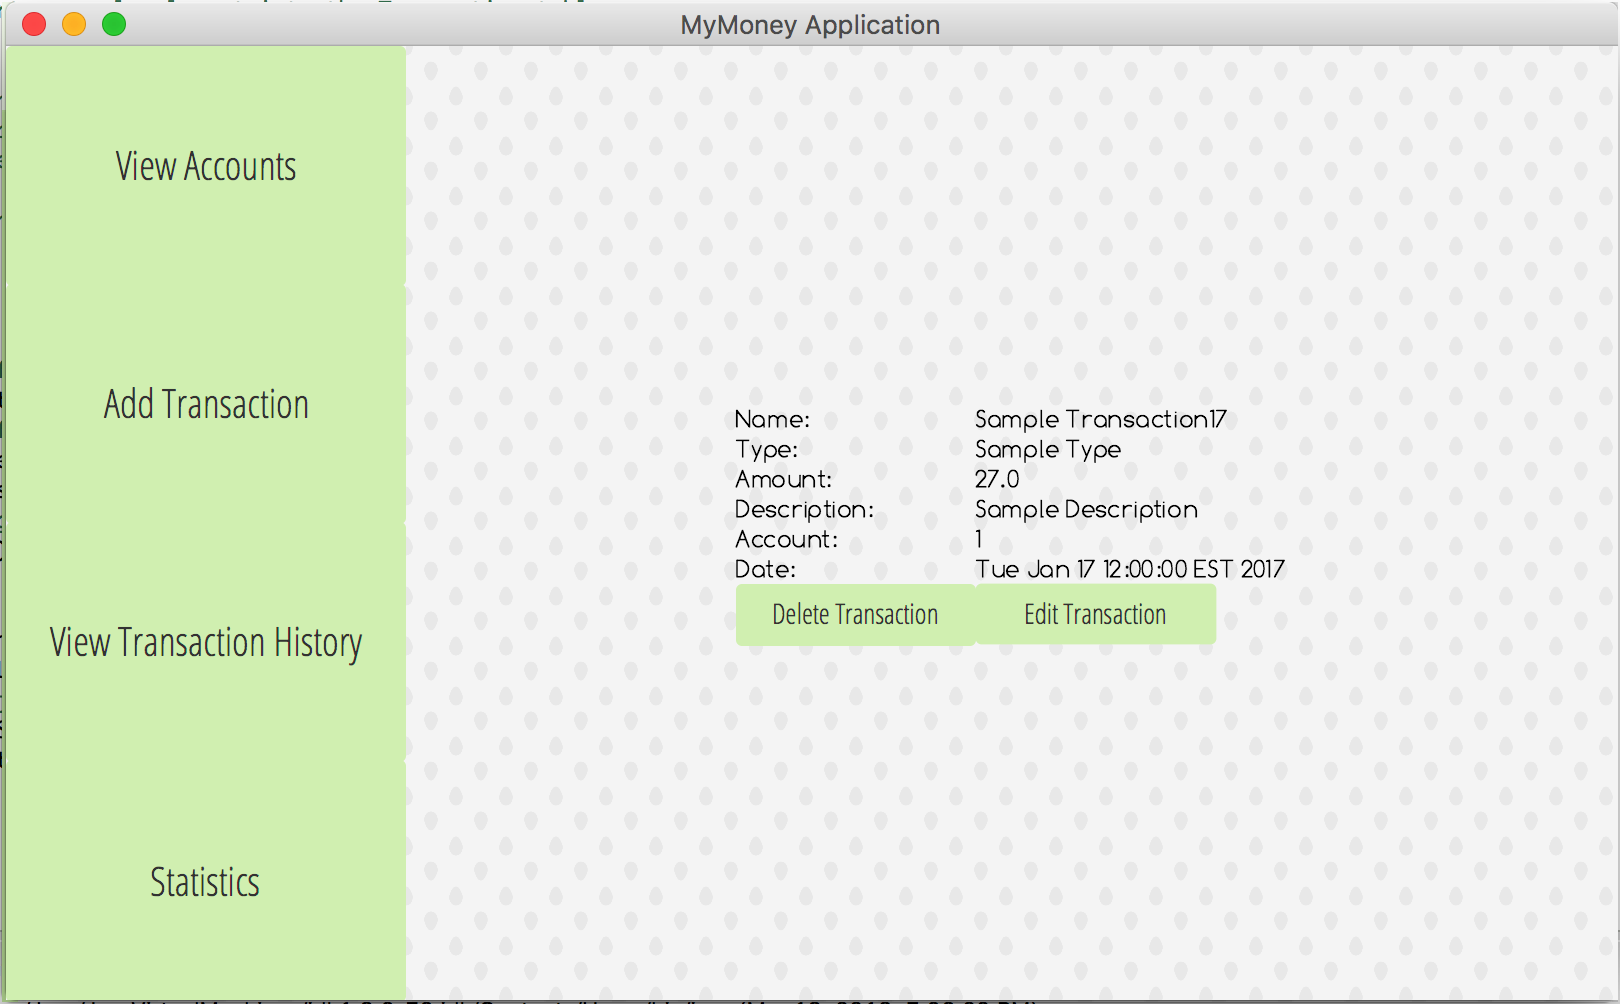
\includegraphics[scale=0.2]{transactiondetail}

The Transaction Detail view displays a full description of the selected
transaction. From this view, the user can see the creation date, and all of the
original data from the creation of the transaction.\\

From the Transaction Detail, the user has two actions: Delete and Edit.
When the user presses delete, the TransactionDetailController's ``deleteTransaction'' method
is called and the transaction is deleted. Once deleted, the user is returned to
the Transaction List view. When the Edit action is invoked, the
TransactionDetailController's ``editTransaction'' method is called which
changes the view to allow all fields to be edited.

\subsubsection{Transaction Add View}

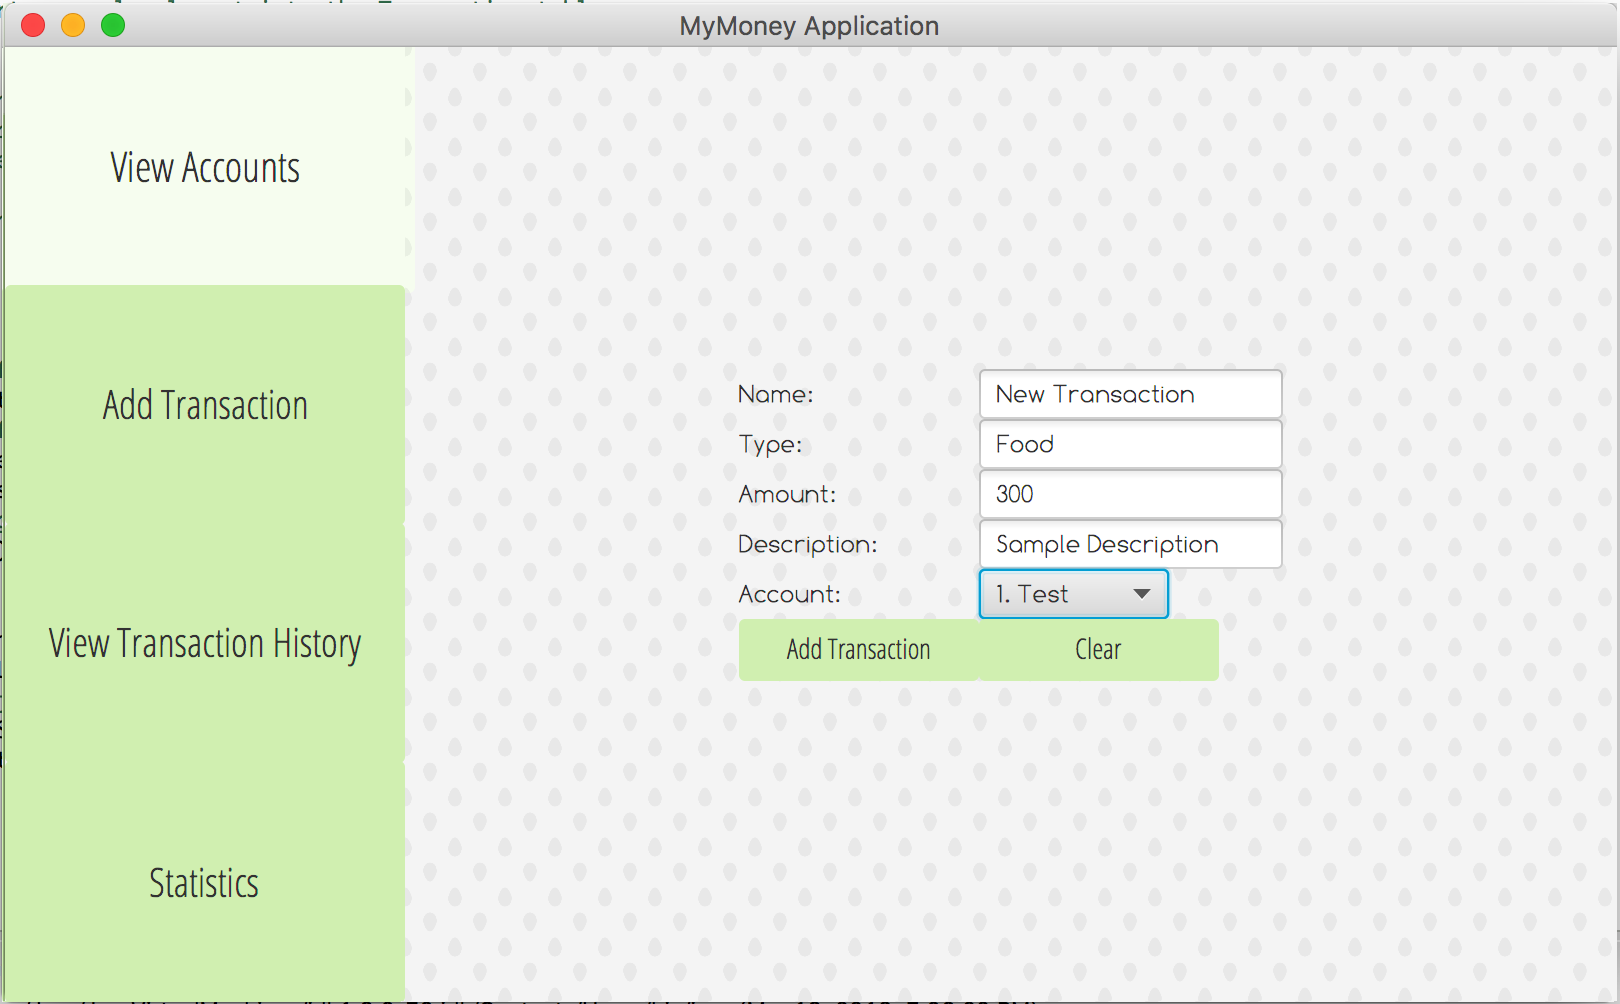
\includegraphics[scale=0.2]{transactionadd}

The Transaction Add view allows the user to add new Transactions to specified accounts.
From the Add view, the user can enter the name, type, amount, description, and associated account
of a transaction and insert it into the database.\\

From the Add view, the user is presented with two actions: Add and Clear.
When Clear is pressed, the TransactionAddController's ``clearTransaction''
method is called which removes any data filled into the view by the user.
The add action calls the ``addTransaction'' method of the TransactionAddController
to insert a new Transaction entry into the database using the TransactionDAO.


\section{Detailed Design} \label{sec:detail}

\subsection{Subsystem X}

\subsubsection{Detailed Design Diagram}

UML class diagram depicting the internal structure of the subsystem,
accompanied by a paragraph of text describing the rationale of this design.

\subsubsection{Units Description}

List each class in this subsystem and write a short description of its purpose,
as well as notes or reminders useful for the programmers who will implement them.
List all attributes and functions of the class.


\section{Dynamic Design Scenarios}

Describe some (at least two) important execution scenarios of the system using UML sequence diagrams.
These scenarios must demonstrate how the various subsystems and units are interacting to achieve a system-level service.
Units and subsystems depicted here must be compatible with the descriptions provided in
section \ref{sec:arch} and \ref{sec:detail}.
`'
\end{document}
